%!TEX root=index.tex
\newacronym{aws}{AWS}{Amazon Web Services}
\newacronym{ec2}{EC2}{Elastic Compute Cloud}
\newacronym{raid}{RAID}{Redundant Array of Independent Disk}
\section{Reference Big Data Framework}
In order to quantitatively process ever increasing amounts of complex data, we need a service framework capable of performing the following operational layers:
\begin{itemize}
	\item retrieving data updates
	\item storing and indexing for optimal retrieval
	\item data discovery and analytics
	\item presenting real-time and offline results
\end{itemize}
All of this must be built on an elastic infrastructure, capable of scaling or shrinking as necessary. Each layer can be represented graphically, building on the layer to its left and on top of some infrastructure implementation. The difference between a framework and a platform is one of flexibility and customization. In order to support a wide variety of future data types and analytic requirements, a framework of tools is preferable to a rigid product solution. Using a framework, it's possible to build loosely coupled layers that can be swapped out as technology evolves. While capable of delivering a superior solution, the cost is is systems integration and development expertise necessary to wire the layers together in a seamless fashion. Figure 1 shows the necessary framework layers. 
\begin{figure}[htbp]
    \centering
    \caption{Framework Layers}
    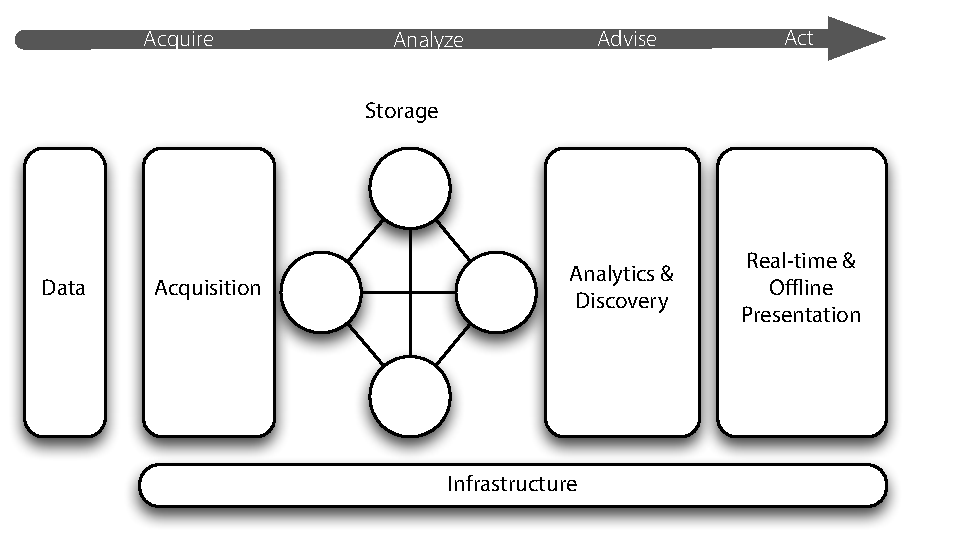
\includegraphics[scale=.80]{framework_layers}
\end{figure}
\subsection{Infrastructure}
At the heart of any big data platform is the elastic infrastructure upon which it is built. The most efficient method of doing this involves virtualization \index{virtualization} of both storage and cpu resources. While \textsc{CSC} has an internal scalable cloud offering known as BizCloud, it has been criticized as being uncompetitive in terms of pricing with the \gls{aws} \index{Amazon Web Services} offering from Amazon [personal communications, 2012]. Infrastructure has two basic fundamental requirements:
\begin{itemize}
    \item cost effectiveness in horizontal scaling
    \item ease of adding, requesting, relinquishing resources
\end{itemize}
Missing from the above list is reliability. Many industry leaders, such as Google, Amazon, Netflix, Twitter, etc, have begun data replication in software as opposed to hardware, moving out of the infrastructure layer and into the individual software stacks. Once implemented, this gives the flexibility to completely replace failed storage and compute nodes with upgraded versions without impacting overall availability. This has the added benefit of dramatically reducing hardware storage costs, since complicated \gls{raid} technology is no longer required to be purchased during every technology refresh. For \climatedge data sets, Linux based \gls{aws} instances coupled to the S3 service are the recommended infrastructure platform.
\subsection{Data Acquisition}
As all the data is freely available via standard HTTP requests, we simply need to put together a framework consisting of a repeatable process that polls each website for newly published data and retrieves it. If necessary, the framework can check with the data store to confirm what is new and what is not. Putting together such a framework is a relatively simple systems integration and development task and has plenty of prior art across the industry. The following components are recommended:
\begin{itemize}
	\item Linux instances to handle retrieval, monitoring, and hosting the source code repository, respectively.
	\item a continuous integration tool, Jenkins or similar, for continually monitoring and notifying the success or failure of the retrieval processes (one per data set). Jenkins will also serve as the means to deploy the most recent code from the code repository onto the server handling the retrieval process. Jenkins is open source and used commonly across the industry for this purpose, resulting in an easily hirable skill set \cite{jenkins}.
	\item a repeatable method, such as Cron, to check and retrieve updated data sets at well defined publication intervals. Jenkins will monitor the success or failure of the cron jobs and notify as needed.
	\item developed code that contacts each web server and pulls down only the most recent data. If the data sets do not offer a simple means of determining what's recent, this code can query the data store so that it's aware of the last stored data. While we need unique code for each data set, the process of determining what's new and retrieving the code should be very similar across all the data sets. It's likely there will a reusable common library of functionality across each specific implementation. This development is likely to be done in a scriptable environment such as Python or Perl. The languages offer an excellent tradeoff between simplicity, flexibility, and execution speed.
\end{itemize}
It is important that this layer elastically scale both in compute and storage capacity as bringing on a new data source, such as \gls{merra}, require substantially more cores to process and disks to hold the raw data while it is prepared for storage. Once the initial loads are done, daily or even monthly loads, should require significantly less capacity.
\subsection{Storing and Indexing}
Once the data has arrived on the local system, it needs to processed and inserted into the data store. This layer is the heart of any service offering. The data store must have the following characteristics:
\begin{itemize}
	\item not inherently possess a single point of failure
	\item horizontally scale (as linearly as possible) in storage and performance
	\item support indexing for realtime and offline analytics
\end{itemize}
There exist several technologies in the top level Apache Hadoop project, one being Cassandra\index{Cassandra}, which fulfill the requirements listed above \cite{cassandra}. There are competing technologies from commercial vendors like EMC, IBM, Intel, SAS, and Oracle, just to name a few, who have similar technologies designed to store and index vast amounts of data. A replication factor of three will help to eliminate single points of failure on the part of the hardware, as well as increase query speed. The tradeoff is the cost to store three times the amount of data.
\subsection{Discovery and Analytics}
The technology behind big data storage is really only interesting to engineers. Customers pay for the results and insights gleaned from analysis of the stored data. This layer makes high usage of the elastic compute infrastructure identified earlier. Analytics generally have two modes in which they are run: realtime and offline. As either set of analytics run, it is crucial to spin up additional capacity as needed, then release it for the cost savings. Through extensive testing and modeling , it should be straightforward to estimate the necessary capacity for all the offline analytics and spin up resources at well established intervals. Realtime is somewhat more difficult as it is difficult to understand the capacity a priori. \gls{ec2} Reserved Instances from \gls{aws} are an excellent way to address this problem. Analytical implementations vary according to specific requirements, but R, Java, or Python are extremely popular and would be ideal for \climatedge.
\subsubsection{Offline Analytics}
Offline analytics, also known as batch, are run at predefined intervals without human interaction. Well defined questions are implemented ahead of time, tested and refined, and then set to run through a scheduling mechanism like Jenkins or Cron. The tornado and flood analytics are excellent examples of a batch jobs needing to be run at well defined intervals to take account of updated data. MapReduce, popularized by Google, is an extremely common implementation of distributed processing over large data sets. It is implementation agnostic and several popular frameworks exist to speed up development. The output from the MapReduce jobs can be stored in the data store and used as input to the presentation layer.
\subsubsection{Realtime Analytics}
Realtime analytics are run on demand, though implementations should make use of as much precomputed data as possible for speed. Since it is not feasible to precompute every possible data combination, the focus is on optimizing commonly accessed data. For example, computing totals, averages, or means for a time period so it is available on demand as a lookup. The tradeoff is between storage and speed. 
\subsection{Presentation}
Any presentation platform must support at least the following formats: \gls{html}, mobile, and XML. Fortunately, wide adoption of \gls{html}5 can render mobile development similar to desktop. Many mobile applications with heavy graphics are still be implemented natively in Objective-C (Apple) or Java (Android), however the performance gap is closing. Javascript rendering of \gls{html} is perhaps the most useful tool for any modern presentation framework.